

\begin{figure*}[t]
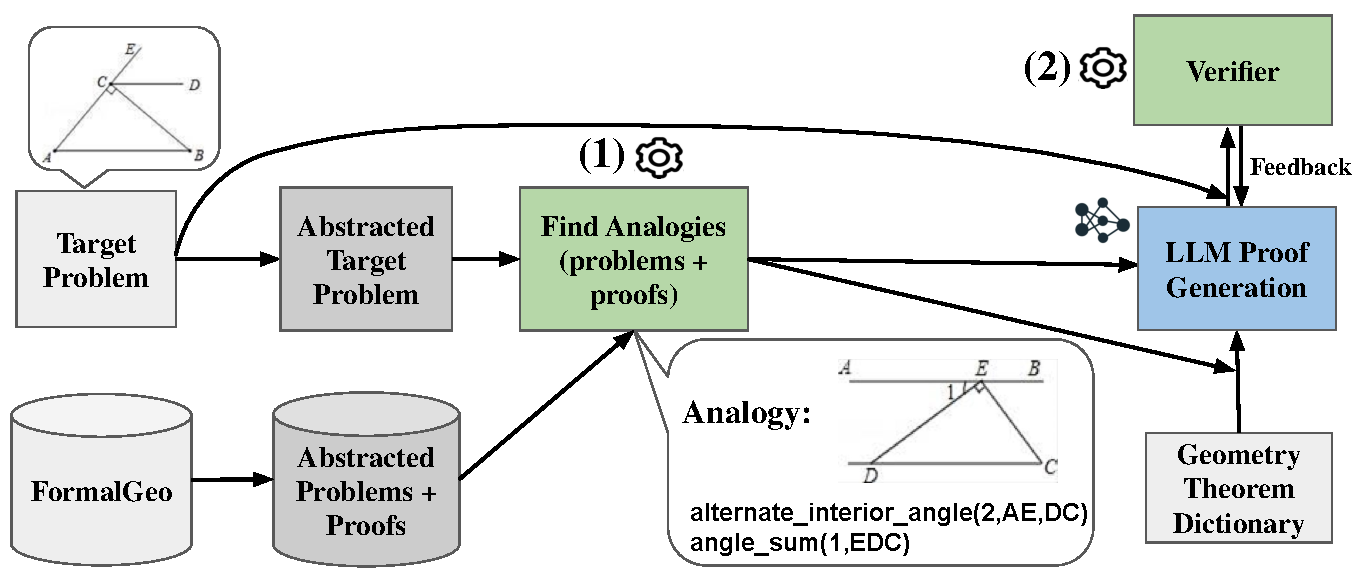
\includegraphics[width=0.9\textwidth]{latex/images/GeometryLLMPipeline.pdf}
\centering
\caption{\textbf{Our neuro-symbolic approach.} Given a target problem from the FormalGeo-7k dataset, we first convert it into an \emph{abstract form} by replacing entity names (e.g., lines, angles) and specific numeric values with placeholders (~\S\ref{subsec:problems_abstraction}).  
We then \emph{retrieve structurally similar problems} from the abstracted dataset by computing Jaccard similarity over key formal components: \textbf{construction} (entities and geometric relations), \textbf{conditions} (e.g., angle equalities, segment lengths), and \textbf{goal} (the conclusion to be proven). This is based on the observation that structurally similar problems often share proof patterns (~\S\ref{subsec:similar_problems_retrieval}).
The retrieved problems, along with their corresponding formal proofs, are presented to an LLM as \emph{in-context examples}, together with the available theorems from the Geometry Theorem Dictionary, to guide \emph{proof generation} for the target problem (~\S\ref{subsec:llm_solver}).  
Finally, a \emph{symbolic verifier} iteratively checks the generated proof and provides feedback until a correct proof is produced or a retry limit is reached (~\S\ref{subsec:verifier}).
}
\label{fig:pipeline}
\end{figure*}



\begin{figure*}[t]
\centering
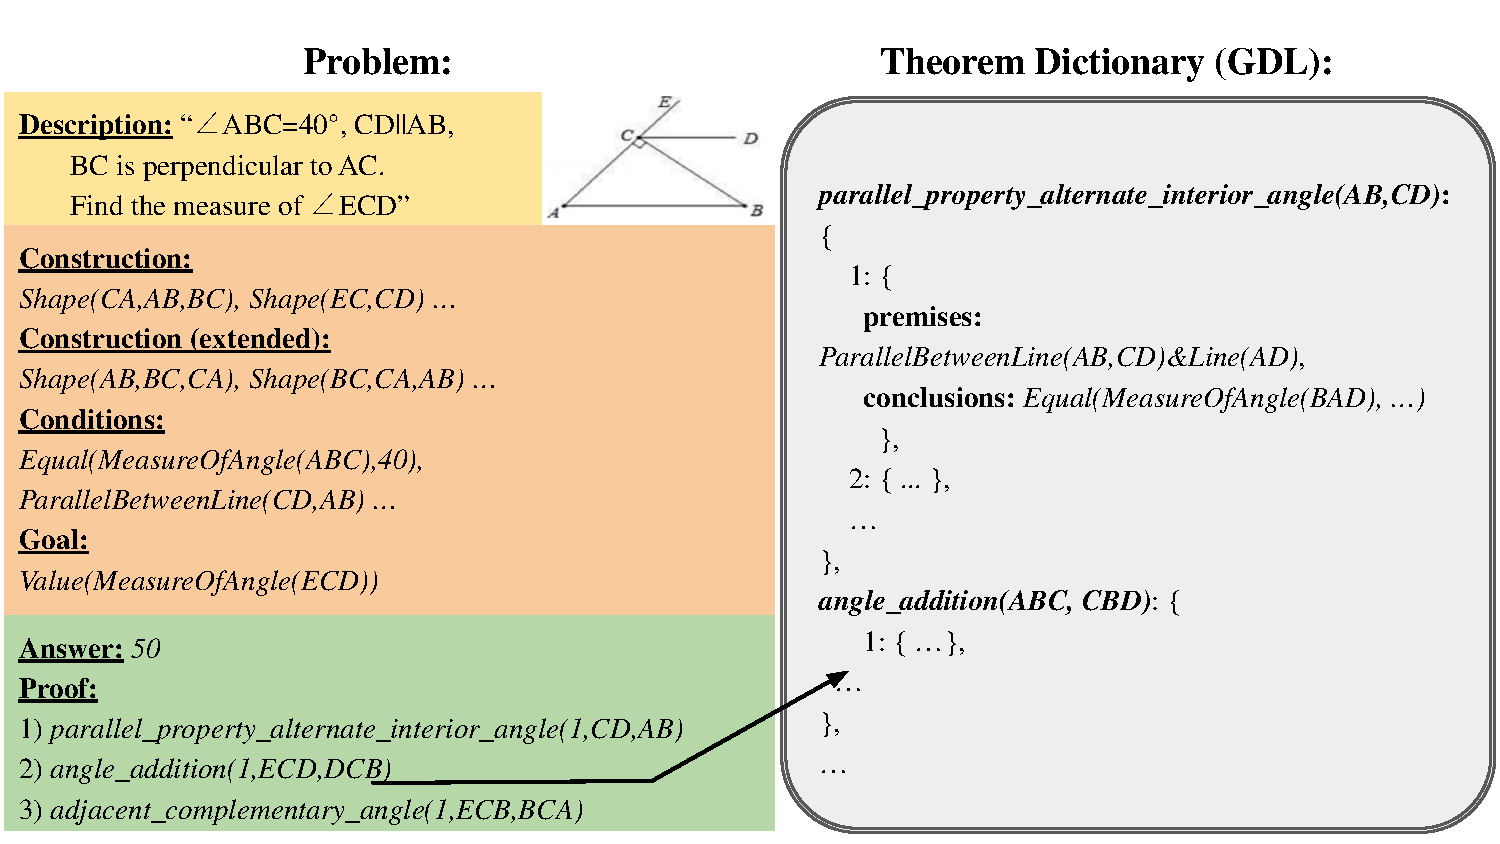
\includegraphics[width=0.9\textwidth]{latex/images/dataset_example.pdf}
\caption{An example problem from FormalGeo-7k.  
\textbf{Left}: Problem inputs, including a natural-language description and formal representations: construction (entities and relations), extended construction (inferred via extension rules), conditions, and goal. The input also includes a numeric answer (or expression) and a formal proof, with each step invoking a theorem from the dictionary.
\textbf{Right}: The Theorem Dictionary, with theorem IDs, arguments, premises, and conclusions. The dataset also includes diagrams (which we do not use), shown here for illustration.
}
\label{fig:dataset_example}
\end{figure*}


% what is the problem

%LLMs have shown remarkable capabilities across a wide range of tasks, from language understanding and generation to code synthesis and problem solving \cite{austin2021program, islam2025codesim, wang2025codevision}.  However, they continue to 
Despite their remarkable performance across a wide range of tasks, LLMs still struggle in formal domains such as mathematical proofs. This stems primarily from their inherent architecture, which relies on probabilistic sequence generation based on patterns 
learned from vast textual datasets.


Mathematical 
proofs demand rigorous logical deduction, symbolic manipulation, and an understanding 
of abstract concepts that go beyond statistical correlations in language. The requirement for absolute 
truth and the absence of ambiguity in mathematical reasoning present a significant challenge for models trained to generate \emph{plausible} text rather than formally valid inferences \cite{singh2024exposing, pan2025lemma}. 
In addition, the often lengthy nature of proofs necessitates a level of sustained logical coherence and hierarchical reasoning 
that is hard for current LLMs. Recent work has shown that altering even superficial aspects of mathematical problems results in significant performance drops \cite{mirzadeh2024gsm}, suggesting that their success often hinges on pattern matching rather than genuine mathematical reasoning.


%\onote{Recent work has further highlighted these limitations: the GSM-8K benchmark \cite{cobbe2021training} was extended to include equivalent variations of math problems, revealing that LLMs show significant performance drops when only superficial aspects like numerical values are altered \cite{mirzadeh2024gsm}. This suggests that their success often hinges on pattern matching rather than genuine mathematical reasoning.}





%that demand rigorous symbolic reasoning, formal notation, and strict logical consistency, such as mathematical proof generation. While LLMs can fluently produce plausible-looking arguments, their outputs are often brittle, error-prone, and difficult to verify \cite{singh2024exposing, jiang2025llms, pan2025lemma}.



% why it is interesting

Enabling LLMs to generate formally verifiable proofs can improve their reliability,\footnote{Throughout this paper, we use \emph{reliable} to refer to the generation of proofs formally verified by a symbolic verifier.} for applications in math, science and education \cite{welleck2022naturalprover, gupta2025beyond, kumar2023math}.
%holds significant promise, with applications in .
%It .
%we just talked about applications, why twice?

% why LLMs, specifically, are a promising route to proof generation

Recent progress demonstrates the promise of LLM-based proof generation. DeepSeek-Prover-V2 achieves state-of-the-art performance in Lean \cite{ren2025deepseek}; AlphaProof and AlphaGeometry 2 reached silver-medal-level performance at IMO 2024, with AlphaGeometry 2 later reaching gold-medalist-level geometry performance \cite{hubert2026olympiad, chervonyi2025gold}; and recent systems have extended formal proof generation to open mathematical research problems and gold-medal-level IMO 2025 performance \cite{tsoukalas2026advancing, achim2025aristotle}.


Unlike specialized automated theorem provers, LLMs can directly process natural-language problem descriptions, draw on broad mathematical knowledge acquired during pretraining, and perform effective heuristic search over the proof space. These qualities motivate our focus on augmenting general-purpose, off-the-shelf LLMs, rather than building or training a domain-specific solver.


% why it is not already been solved?


%The challenge lies with \dnote{?} the fundamental nature of LLMs, which are trained to model patterns in natural language using probabilistic sequence prediction. As a result, their outputs, while often fluent, tend to lack the precision, structure, and symbolic rigor required for formal reasoning. 

%Natural-language proofs are typically ambiguous and hard to verify with symbolic verification tools.


%One alternative is to generate proofs directly in formal language, but this demands absolute logical validity, symbolic manipulation, and hierarchical reasoning over long contexts --  
% capabilities that remain particularly difficult for current LLMs. As a result, verifying LLM-generated proofs reliably and automatically remains challenging.




% what we propose


In this work, we introduce a neuro-symbolic approach that combines the generative strengths of LLMs with two complementary structured components: (1) \textbf{analogical guidance} and (2) \textbf{symbolic verification}. See Figure~\ref{fig:pipeline} for an illustration.

The first component retrieves analogous problems and their proofs to guide the model. This is inspired by cognitive science, where analogy is recognized as fundamental to human problem-solving and generalization \cite{gentner1983structure, holyoak1996mental}, as well as recent work showing that prompting LLMs to generate analogous problems and solutions can improve performance on math problems \cite{yasunaga2023large}.

Our central hypothesis is that \emph{structurally analogous geometry problems admit similar proofs}. Since the target proof is unavailable at inference time, we construct abstract symbolic representations of problem statements and learn to predict proof similarity from these features. Retrieved proofs of analogous problems then provide useful starting points for proof generation and help identify the most relevant theorems to present to the model, substantially reducing costs.
%leverages the hypothesis that structurally similar problems tend to yield similar proofs. By r


To complement this, our second component employs a symbolic verifier that checks the generated proofs and provides structured feedback. This feedback drives an iterative loop, enabling the model to revise its output until a valid proof is obtained. 
%Together, these components form a closed-loop system where proof generation is guided by prior solutions and the solution is formally verified. 



As a proof of concept, we focus on Euclidean geometry -- a symbolic, verifiable domain rich in structural analogies.
Our goal is to evaluate whether our symbolic augmentations improve the proof-generation capabilities of \emph{general-purpose LLMs}. Thus, while we use geometry as our testbed, our focus is \emph{not} on competing with specialized state-of-the-art geometry solvers, but rather on quantifying the gains enabled by our method.
%We show that our approach significantly improves proof accuracy for OpenAI’s o1 model (58\%-70\% improvement).
%Importantly, we find that both components of our method -- analogy guidance and the verifier -- provide complementary gains in performance.
%We hope our results will inspire further work 
%on developing neuro-symbolic methods for mathematical reasoning.
\textbf{Our main contributions are:}
\textbf{(1)} We propose a neuro-symbolic system that aids LLMs in proof generation by providing analogical guidance and verification feedback.
\textbf{(2)} We design a symbolic verifier tailored to geometry proofs with expressive feedback. In contrast to other works, we evaluate the {\bf entire proof}, not just the final numeric answer.
%, allowing us to assess the model’s reasoning process.}
\textbf{(3)} Our method substantially improves proof accuracy across all models while reducing computational cost through focused context construction. Our complete pipeline achieves 68\%-96\% accuracy, compared with 10\%-44\% for LLM-only baselines. Under matched inference budgets with verifier feedback, analogical guidance improves accuracy from 88\% to 96\% for GPT-5, 78\% to 86\% for Claude Sonnet 4.6, 72\% to 86\% for Gemini-Flash-2.5, and 52\% to 80\% for o1. At the same time, it substantially reduces the theorem dictionary size (e.g., from 18K to 2.5K tokens on average for o1).
\textbf{(4)} We release data and code at: \url{https://github.com/orensul/LLMs_proof_generation}.
 
%, saving 0.23\$ per API call to OpenAI's o1 model.
% 17950 tokens -- all dictionary. 2513 tokens -- abridged dictionary



% This limitation arises from the fundamental nature of LLMs, which are trained to model patterns in natural language using probabilistic sequence prediction. In contrast, mathematical proofs demand absolute logical validity, symbolic manipulation, and hierarchical reasoning over long contexts. These requirements go beyond the surface-level coherence LLMs typically optimize for, and introduce challenges such as ensuring factual correctness, avoiding ambiguity, and maintaining long-range logical consistency. 



% In formal mathematical reasoning, where truth is binary and even minor deviations can render a proof invalid, the inability to ensure rigorously correct outputs remains a central challenge in deploying LLMs. A proof must be flawless and verifiable by an automated verifier to be considered valid \cite{cobbe2021training, wang2023mathshepherd}.
